% !TEX TS-program = pdflatex
% !TEX encoding = UTF-8 Unicode

% This is a simple template for a LaTeX document using the "article" class.
% See "book", "report", "letter" for other types of document.

\documentclass[11pt,titlepage]{article} % use larger type; default would be 10pt

\usepackage[utf8]{inputenc} % set input encoding (not needed with XeLaTeX)

%%% Examples of Article customizations
% These packages are optional, depending whether you want the features they provide.
% See the LaTeX Companion or other references for full information.

%%% PAGE DIMENSIONS
\usepackage{geometry} % to change the page dimensions
\geometry{a4paper} % or letterpaper (US) or a5paper or....
% \geometry{margin=2in} % for example, change the margins to 2 inches all round
% \geometry{landscape} % set up the page for landscape
%   read geometry.pdf for detailed page layout information

\usepackage{graphicx} % support the \includegraphics command and options
\usepackage{titlepic}

% \usepackage[parfill]{parskip} % Activate to begin paragraphs with an empty line rather than an indent

%%% PACKAGES
\usepackage{booktabs} % for much better looking tables
\usepackage{array} % for better arrays (eg matrices) in maths
\usepackage{paralist} % very flexible & customisable lists (eg. enumerate/itemize, etc.)
\usepackage{verbatim} % adds environment for commenting out blocks of text & for better verbatim
\usepackage{subfig} % make it possible to include more than one captioned figure/table in a single float
% These packages are all incorporated in the memoir class to one degree or another...

%%% HEADERS & FOOTERS
\usepackage{fancyhdr} % This should be set AFTER setting up the page geometry
\pagestyle{fancy} % options: empty , plain , fancy
\renewcommand{\headrulewidth}{0pt} % customise the layout...
\lhead{}\chead{}\rhead{}
\lfoot{}\cfoot{\thepage}\rfoot{}

%%% SECTION TITLE APPEARANCE
\usepackage{sectsty}
\allsectionsfont{\sffamily\mdseries\upshape} % (See the fntguide.pdf for font help)
% (This matches ConTeXt defaults)

%%% ToC (table of contents) APPEARANCE
\usepackage[nottoc,notlof,notlot]{tocbibind} % Put the bibliography in the ToC
\usepackage[titles,subfigure]{tocloft} % Alter the style of the Table of Contents
\renewcommand{\cftsecfont}{\rmfamily\mdseries\upshape}
\renewcommand{\cftsecpagefont}{\rmfamily\mdseries\upshape} % No bold!

\newenvironment{changemargin}[3]{%
\begin{list}{}{%
\setlength{\topsep}{0pt}%
\setlength{\headsep}{#3}%
\setlength{\leftmargin}{#1}%
\setlength{\rightmargin}{#2}%
\setlength{\listparindent}{\parindent}%
\setlength{\itemindent}{\parindent}%
\setlength{\parsep}{\parskip}%
}%
\item[]}{\end{list}}

%Table Formatting
\usepackage{tabularx,hhline}
\usepackage{pbox}
\usepackage{booktabs}
\usepackage{makecell}
\usepackage{float}

%%% END Article customizations

%%% The "real" document content comes below...

\titlepic{
\includegraphics[scale=0.60]{polimi_logo.jpg}}
\title{Project Plan Document \\ \vspace{1cm} \large{Version 1.0}}
\author{Giorgio Pea(Mat. 853872), Andrea Sessa(Mat. 850082)}
\date{2/2/2016}

\begin{document}

\maketitle

\newpage

\tableofcontents

\newpage

\section{Introduction}
  \subsection{Purpose}
    The main purpose of this document is to analyze effort and cost for MyTaxiService.
    The analisys is performed using two different models:
    \begin{itemize}
     \item Function Points: to determine the size and the overall complexity of the project
     \item COCOMO II: to determine the effort and cost of the project
    \end{itemize}
    In the final part of the document are also included a Gantt diagram to visualize thepage
    general schedule of the project and a resource allocation diagram to show how the team 
    members have been assigned to the variuos tasks.

  \subsection{Acronyms}
    \begin{itemize}
     \item \textbf{RASD:} Requirements Analisys and Specification Document
     \item \textbf{DD:} Design Document
     \item \textbf{ITPD:} Integration Test Plan Document
     \item \textbf{AWT:} Approximate Waiting Time
    \end{itemize}
  \subsection{References}
    \begin{itemize}
     \item 
    \end{itemize}

\section{Function Point Analisys}
  \subsection{Internal Logic Files}
     The system needs to store information about: \newline \newline
     \textbf{User}\newline
     This data entity consist in a small set of information, for this reason its complexity has been considered \textbf{SIMPLE}\newline\newline
     \textbf{Administrator}\newline
     This data entity consist in a small set of information, for this reason its complexity has been considered \textbf{SIMPLE}\newline\newline
     \textbf{Mtaxi driver}\newline
     This data entity consist in a small set of information, for this reason its complexity has been considered \textbf{SIMPLE}\newline\newline
     
     \newpage
     
     \noindent \textbf{Mtaxi}\newline
     This data entity consist in a small set of information, for this reason its complexity has been considered \textbf{SIMPLE}\newline\newline
     \textbf{WorkTime Table}\newline
     This data entity consist in a small set of information, for this reason its complexity has been considered \textbf{SIMPLE}\newline\newline
     \textbf{Zone}\newline
     This data entity consist in a small set of information, for this reason its complexity has been considered \textbf{SIMPLE}\newline\newline
     \textbf{Location}\newline
     This data entity consist in a small set of information, for this reason its complexity has been considered \textbf{SIMPLE}\newline\newline
     \textbf{Ride Request} 
     This data entity consist in a small set of information, for this reason its complexity has been considered \textbf{SIMPLE}\newline\newline
     \textbf{Booking Request}
     This data entity consist in a small set of information, for this reason its complexity has been considered \textbf{SIMPLE}\newline\newline
     \textbf{Queue}
     This data entity consist in a small set of information, for this reason its complexity has been considered \textbf{SIMPLE}\newline
     
     \begin{center}
      $ ILF Function Points = numberOfILF * 7 = 7 * 7 = 49 $
     \end{center}

   \subsection{External Logic Files}
    The system needs to access data about:\newline\newline
    \textbf{External Traffic data}\newline
    The structure of this data could be complex and could need a digest process, for this reason its complexity has been considered \textbf{MEDIUM}\newline
    
    \begin{center}
     $ ILF Function Points = numberOfELF * 7 = 1 * 7 = 7 $
    \end{center}
    
    \subsection{External Input}
     The system needs to process the following input: \newline

      \noindent \textbf{Ride Request creation}\newline
      This operation requires the user to perform few and simple actions and the system to perform straightforward checks and data procedures,
      for this reason its complexity has been considered \textbf{SIMPLE}\newline\newline
      
      \noindent \textbf{Booking Request creation}\newline
      This operation requires the user to perform few and simple actions and the system to perform straightforward checks and data procedures,
      for this reason its complexity has been considered \textbf{SIMPLE}\newline\newline
      
      \noindent \textbf{Booking Request editing}\newline
      This operation requires the user to perform few and simple actions and the system to perform straightforward checks and data procedures,
      for this reason its complexity has been considered \textbf{SIMPLE}\newline\newline
      
      \noindent \textbf{User Login/Logout}\newline
      This operation requires the user to perform few and simple actions and the system to perform straightforward checks and data procedures,
      for this reason its complexity has been considered \textbf{SIMPLE}\newline\newline
      
      \noindent \textbf{User Registration}\newline
      This operation requires the user to perform few and simple actions and the system to perform straightforward checks and data procedures,
      for this reason its complexity has been considered \textbf{SIMPLE}\newline\newline
      
      \noindent \textbf{Mtaxi Driver Registration}\newline
      This operation requires the Mtaxi driver to perform few and simple actions and the system to perform straightforward checks and data procedures,
      for this reason its complexity has been considered \textbf{SIMPLE}\newline\newline
      
      \noindent \textbf{Driver Notification}\newline
      This operation requires the user to perform few and simple actions and the system(including the MYT device) more complex and numerous procedures,
      for this reason its complexity has been considered \textbf{MEDIUM}\newline\newline
      
      \noindent \textbf{Administrator Operations}\newline
      This operation requires the administrator to perform few and simple actions and the system to perform straightforward checks and data procedures,
      for this reason its complexity has been considered \textbf{SIMPLE}\newline
      
      \begin{center}
	$ EI Function Points = numberOfSimpleEI * 3 + numberOfMediumEI * 4 = 7 * 3 + 1 * 4 = 25 $
      \end{center}
    
    \subsection{External Output}
      This operation requires the system to perform complex calculations on traffic data and Mtaxi positions, for this reason its complexity has been considered \textbf{COMPLEX}\newline\newline
      \textbf{AWT Notification}\newline
      
      \textbf{Zone Change Notification}\newline
      This operation implies that the system noticed an unbalanced distribution of Mtaxi in city zones; this last process requires complex and numerous
      calculations and data checks, this operation requires the system to perform complex calculations on traffic data and Mtaxi positions, for this reason its complexity has been considered \textbf{COMPLEX}\newline
      \begin{center}
	$ EO Function Points = numberOfEO * 7 = 2 * 7 = 14 $
      \end{center}
      
    \subsection{External Inquiry}
       \textbf{User Profile Visualization}\newline
       This operation the system to retrieve and elaborate data in a simple way, for this reason its complexity has been considered \textbf{SIMPLE}\newline\newline
       \textbf{User Ride Request Visualization}\newline
       This operation the system to retrieve and elaborate data in a simple way, for this reason its complexity has been considered \textbf{SIMPLE}\newline\newline
       \textbf{User Booking Request Visualization}\newline
       This operation the system to retrieve and elaborate data in a simple way, for this reason its complexity has been considered \textbf{SIMPLE}\newline\newline
       \textbf{Mtaxi Notification Visualization}\newline
       This operation the system to retrieve and elaborate data in a simple way, for this reason its complexity has been considered \textbf{SIMPLE}\newline\newline
       \textbf{Mtaxi Accident Reports Visualization}\newline
       This operation the system to retrieve and elaborate data in a simple way, for this reason its complexity has been considered \textbf{SIMPLE}\newline\newline
       \newpage
       \textbf{Mtaxi Bad Behavior Reports Visualization}\newline
       This operation the system to retrieve and elaborate data in a simple way, for this reason its complexity has been considered \textbf{SIMPLE}\newline
       \begin{center}
	$ EI Function Points = numberOfEI * 3 = 6 * 3 = 18 $
       \end{center}
     
     \subsection{Summary}
	\begin{center}
	$ Total Function Points = 49 + 7 + 25 + 14 + 18  = 113 $
        $ Number of SLOC = JavaFPConversionFactor * TFP = 46 * 113 = 5198 \: SLOCs $
	\end{center}

\newpage
\section{COCOMO II Analisys}

\newpage

\section{Task Gantt Diagram}
 In this section is included a gantt diagram that represents the tasks in which the project is divided.\newline
 \begin{center}
  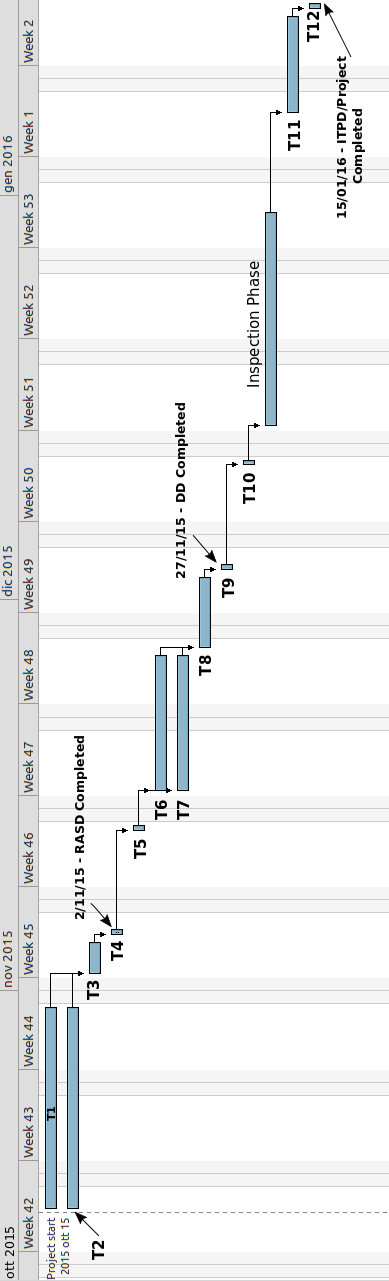
\includegraphics[scale=0.4]{gantt.png}
 \end{center}
\newpage

In the following paragraph is included an explanation of each task and of its duration in terms of work
\begin{itemize}
 \item \textbf{T1:} Requirements Specification - Duration: 29h
 \item \textbf{T2:} RASD Diagrams Specification - Duration: 29h
 \item \textbf{T3:} Alloy Model Definition - Duration: 4h
 \item \textbf{T4:} RASD Revision - Duration: 2h
 \item \textbf{T5:} RASD Post-Presentation Revision - Duration: 2h
 \item \textbf{T6:} Architecture Specification - Duration: 18h
 \item \textbf{T7:} DD Diagrams Specification - Duration: 18h
 \item \textbf{T8:} Algorithms Definition - Duration: 2h
 \item \textbf{T9:} DD Revision - Duration: 2h
 \item \textbf{T10} DD Post-Presentation Revision - Duration: 2h
 \item \textbf{T11:} Integration Test Plan Definition - Duration: 8h
 \item \textbf{T12:} ITPD Revision: Duration: 1h
\end{itemize}

\newpage
\section{Resource Allocation Diagram}

\section{Appendix}

\end{document}
